\documentclass[10pt,letterpaper]{memoir}
% memoir commands to define the text block geometry
\setulmarginsandblock{1in}{*}{*}
\setlrmarginsandblock{1in}{*}{*}

\usepackage{xparse}
\usepackage{blindtext}
\usepackage{enumitem}
\usepackage{graphicx}

\usepackage{amsmath,mathtools,amssymb}
% See https://texblog.net/latex-archive/maths/amsmath-matrix/ 
% for an explanation of this extention of the amsmath matrix commands.
% It's a way to enable "augmented matrices" using a new optional argument:
%
% \begin{pmatrix}[cc|c]
%     1 & 2 & 3\\
%     4 & 5 & 9
%   \end{pmatrix}
%
\makeatletter
\renewcommand*\env@matrix[1][*\c@MaxMatrixCols c]{%
  \hskip -\arraycolsep
  \let\@ifnextchar\new@ifnextchar
  \array{#1}}
\makeatother

\usepackage{bm} % bold math package

\usepackage{booktabs}
\usepackage{multirow}
\usepackage{hyperref}
\usepackage{systeme}

\usepackage{tcolorbox}
    \tcbuselibrary{skins}
    \tcbuselibrary{raster}
    \tcbuselibrary{skins}
\usepackage{tikz}
    \usetikzlibrary{arrows.meta}
\usepackage{tkz-base}
\usepackage{tkz-fct}    
\usepackage{pgfplots}
    \pgfplotsset{compat=newest}

% for inserting blanks that the students fill in
\usepackage{dashundergaps} % for \gap
\dashundergapssetup{
    teacher-mode=false, % set to true to show answers 
    gap-format=underline,
    teacher-gap-format=underline,
    gap-font={\ECFAugie\MTversion{augie}\color{black}},
    gap-numbers=false,
    gap-widen=true,
    gap-extend-percent=100, % note: making this too big might create errors
    gap-number-format=\,\textsuperscript{\normalfont(\thegapnumber)},
}

\usepackage{emerald}
\usepackage[subdued]{mathastext}% no italic for Augie anyhow
    \MTDeclareVersion[n]{lmvtt}{T1}{lmvtt}{m}{n}
    \MTfamily{augie}
    \Mathastext[augie]

\newcommand{\myHeadFootStyle}{\footnotesize\sffamily}
\copypagestyle{myPagestyle}{empty}
%
% FIXME
% The following header definitions do NOT work right in all cases.
% I have found that the chapter title sometimes gets picked up from
% a chapter that begins on the NEXT PAGE. Not sure what's going on.
% So I abandoned embedding the info in the header and instead updated
% \myLesson to print it out, and that seems to work find.
%
% \makeoddhead{myPagestyle}
%     {\,}
%     {\,}
%     {\myHeadFootStyle\chaptername\,\thechapter\,\,\myCurrentChapterTitle}
% \makeevenhead{myPagestyle} 
%     {\,}
%     {\,}
%     {\myHeadFootStyle\chaptername\,\thechapter\,\,\myCurrentChapterTitle}
\makeoddfoot{myPagestyle}
    {\myHeadFootStyle\myCurrentBookTitle}
    {\myHeadFootStyle\thepage}
    {\myHeadFootStyle\thechapter.\themyLessonCounter\,\,\myCurrentLessonTitle}
\makeevenfoot{myPagestyle}
    {\myHeadFootStyle\thechapter.\themyLessonCounter\,\,\myCurrentLessonTitle}
    {\myHeadFootStyle\thepage}
    {\myHeadFootStyle\myCurrentBookTitle}


\setlength{\parindent}{0em}
\setlength{\parskip}{0.75em}

\begin{document}
\pagestyle{plain}
\checkandfixthelayout
% \raggedbottom
\dashundergapssetup{teacher-mode=false,}

\newcommand{\myEmph}{\bfseries\itshape}
\newcommand{\myClassName}{{\tagged{pre-AP}{pre-AP }}Algebra 2}

% So I can save/restore \fboxsep
\newlength{\mySavedFboxsep}
\newcommand{\mySaveFboxsep}{\setlength{\mySavedFboxsep}{\fboxsep}}
\newcommand{\mySaveAndSetFboxsep}[1]{
    \setlength{\mySavedFboxsep}{\fboxsep}
    \setlength{\fboxsep}{#1}
}
\newcommand{\myRestoreFboxsep}{\setlength{\fboxsep}{\mySavedFboxsep}}

% A centered tcolorbox
%
% #1 - options to pass to tcolorbox
%
\NewDocumentEnvironment{myCenteredBox}{m}{%
    \begin{center}
    \begin{tcolorbox}[#1]
}{
    \end{tcolorbox}
    \end{center}
}


% A centered system of equations
%
\NewDocumentCommand{\myCenteredSysteme}{m}{%
    \begin{center}\systeme{#1}\end{center}
}

%
% This specialized command is my way of typesetting a table for
% students to use when solving systems of equations using matrices.
%
% - I make it really wide, because I need horizontal space. The increase in margin width 
%   is adjustable, but frankly, there are a lot of hard-coded dimensions in the table, so
%   I'm not positive that generality works well.
%
% - I put the content in a tikz picture with an OPAQUE background, since I 
%   plan to overlay this on top of Examples, which have dotted boxes around 
%   them at the "normal" margins.
%
% - The table uses the multirow package so that I can have the "Solution" box span two cells.
%
\NewDocumentCommand{\myWideMatrixTable}{O{-0.7in}}{
    \begin{adjustwidth}{#1}{#1}
        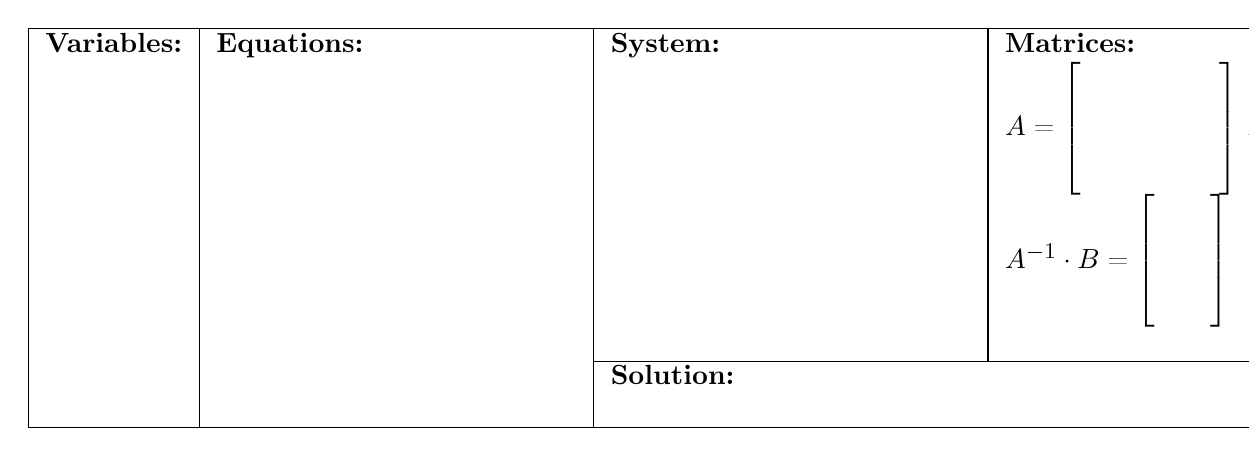
\begin{tikzpicture}
            \node
            [
                text width=1.25\textwidth, %I dinked with the multiplier to get balanced margins
                fill=white!30, 
                fill opacity=1,
                text opacity=1,
                inner sep=0pt,
            ]
            {%
                \begin{tabular}{|l|m{1.8in}|m{1.8in}|m{2.1in}|}
                    \hline
                    {\bfseries\scshape Variables:} & {\bfseries\scshape Equations:} & {\bfseries\scshape System:} & {\bfseries\scshape Matrices:} \\
                    % & & & \\
                    & & & 
                    \(
                        A = 
                        \begin{bmatrix}
                            \phantom{99} & \phantom{99} & \phantom{99} \\
                            \phantom{99} & \phantom{99} & \phantom{99} \\
                            \phantom{99} & \phantom{99} & \phantom{99} \\
                            \phantom{99} & \phantom{99} & \phantom{99} \\
                        \end{bmatrix}
                    \)
                    \(
                        B = 
                        \begin{bmatrix}
                            \phantom{999}\\
                            \phantom{999}\\
                            \phantom{999}\\
                            \phantom{999}\\
                    \end{bmatrix}
                    \)
                    \\
                    & & &
                    \(
                        A^{-1}\cdot B = 
                        \begin{bmatrix}
                            \phantom{9999}\\
                            \phantom{999}\\
                            \phantom{999}\\
                            \phantom{999}\\
                    \end{bmatrix}
                    \)
                    \\
                    & & & \\ \cline{3-4}
                    & & 
                    \multicolumn{2}{l|}{\bfseries\scshape Solution:}
                    \\ 
                    & & 
                    \multicolumn{2}{l|}{\,}
                    \\ 
                    \hline
                \end{tabular}
            };
        \end{tikzpicture}
    \end{adjustwidth}
}


{\small Pre-AP Algebra 2}\hfill Name: \rule{2in}{0.15mm}

{\bfseries\Large PAP HW 4.6 Linear Regression}\hfill Period: \rule{0.5in}{0.15mm}

In the following problems, 
you will use {\bfseries\itshape linear regression} to find the 
``best fit'' line for some real world data.
\begin{itemize}[noitemsep,parsep=0in]
    \item the horizontal axis is time {dates}, and
    \item the vertical axis is the performance of computer chips.
\end{itemize}


{\Large\bfseries Problem 1)}{\itshape Intel chip performance vs. time}

Enter these data into a table in the {\scshape Desmos graphing calculator}.
\begin{center}
    \begin{tabular}{cc}
        \toprule
            release date & Intel chip \\
            & performance (SPECint2006) \\
        \midrule
            2014.25 & 41.4 \\
            2015.25 & 41.4 \\
            2015.50 & 45.6 \\
            2017.00 & 49.2 \\
            2018.75 & 54.3 \\
            2020.25 & 58.6 \\
            2020.75 & 55.3 \\
        \bottomrule
    \end{tabular}
\end{center}
The column names for the {\scshape Desmos} table should be $x_1$ and $y_1$.

Use {\scshape Desmos} the find the best fit line for these data using regression.
(Type \texttt{y1 $\sim$ m1 x1 + b1} into a new formula just after the table.)\footnote{
    We're using $m_1$ and $b_1$ so that we don't mix them up with the slope and intercept 
    for a second regression we do below.
}

Write down the slope and intercept of that line:\quad 
$m_1$ = \gap{\phantom{99.999}}\qquad$b_1$ = \gap{\phantom{99.999}}


\vspace{3em}
{\Large\bfseries Problem 2)}{\itshape Apple/ARM chip performance vs. time}

Enter these data into a {\bfseries\itshape second}
table in the {\scshape Desmos graphing calculator}.
\begin{center}
    \begin{tabular}{cc}
        \toprule
            release date & Apple/ARM chip\\
            & performance (SPECint2006) \\
        \midrule
            2015.75 & 21.1 \\
            2016.75 & 28.7 \\
            2017.75 & 36.8 \\
            2018.75 & 45.3 \\
            2019.75 & 54.9 \\
            2020.75 & 63.3 \\
        \bottomrule
    \end{tabular}
\end{center}
The column names for the {\scshape Desmos} table should be $x_2$ and $y_2$.

Use {\scshape Desmos} the find the best fit line for these data using regression.
(Type \texttt{y2 $\sim$ m2 x2 + b2} into a new formula just after the table.)\footnote{
    We're using $m_2$ and $b_2$ so that we don't mix them up with the slope and intercept 
    from the regression we did above.
}

Write down the slope and intercept of that line:\quad
$m_2$ = \gap{\phantom{99.999}}\qquad$b_2$ = \gap{\phantom{99.999}}



\newpage
{\Large\bfseries Problem 3)}{\itshape chip performance comparison}

Plot the two lines on the same {\scshape Desmos} graph.
({\scshape Desmos} probably did it for you already!)
Find the coordinates of the intersection of the two lines:\\[1.5em]
$x$ (date) = \gap{\phantom{9999.999}}\qquad$y$ (performance) = \gap{\phantom{99.99}}

Sketch the two lines and their point of intersection below.
\vspace{2in}




\vspace{3em}
{\Large\bfseries Problem 4)}{\itshape disruption}

Apple started making {\itshape iPhones} in 2007.
When they started, Apple asked Intel 
(who made the chips in Apple's Mac laptop and desktop computers)
if they would like to make the chip in the new Apple phone.
Intel said, ``No.''
They didn't think there would be enough phones for them to make money doing it.

{\itshape Big mistake.}

So Apple started designing their own chips.
Over the years (as you can see on the graph from the second table),
Apple's chips got faster and began approaching Intel's chip performance.

Very recently (in the last couple weeks),
Apple announced that they are {\bfseries\itshape phasing out} Intel chips
from all their computers. 
Apple chips are now faster (and use less power, so they are cooler) than Intel chips.
Apple's ARM designs are now a {\bfseries\itshape big threat} to Intel's dominance 
in the computer chip design business.

Your graph in the last problem shows where the ``cross-over point'' is---when 
Apple's chips finally reached the same level of performance as Intel's.

In the business world, this is known as {\LARGE\bfseries\itshape disruption}
where a dominant company's business is challenged by the emergence 
of an unexpected competitor.
(Apple was an unexpected competitor to Intel.)

Ok, so here's the question (finally!)\dots

Assuming Apple started designing ARM chips in 2007 (when they first released the {\itshape iPhone}),
according to your graph in the last problem,
how long did it take until Apple disrupted Intel?
(How long did it take to get to the ``crossover point''?)

It took approximately \gap{99.99} years.
Briefly explain how you got that answer.

\end{document}